\documentclass[handout]{beamer}
 
\usepackage[utf8]{inputenc}
\usepackage{mathtools}
\usepackage{tikz}
\usetikzlibrary{calc}

\usetheme{CambridgeUS}
\useoutertheme{split}
\setbeamertemplate{title page}[default][colsep=-4bp,rounded=true]
 
%Information to be included in the title page:
\title{Message Integrity}
\author{Rohit Musti}
\institute{CUNY - Hunter College}
\date{\today}
 
\begin{document}
 
\frame{\titlepage}

\begin{frame}
    \frametitle{Message Integrity Motivation}
    \begin{itemize}
      \item \pause Up until now we have considered \textit{passive} actors, who observe but do not attempt to modify messages \pause
      \item What about \textit{active} actors who are trying to modify the messages before they're recieved? Do any examples come to mind? \pause
      \item Imagine you are delivering stock information to the public information. The message secrecy is not important (everyone is allowed to know the contents of the message), but message integrity is very important! \pause
      \item Imagine you are delivering the results of medical tests to a patient, the message secrecy is important and the message integrity is (a mis-diagnosis can have massive ramifications)! \pause
      \item Imagine you are downloading open source software online, it is extremely important to be able to verify that the software you downloaded is the correct source

    \end{itemize}

\end{frame}


\begin{frame}
    \frametitle{Man in the Middle Attack}
    \pause \text{Let \(\mathcal{E} = (E, D) \) be a cipher secure against chosen plaintext attacks}\\ \pause
    \bigskip
    \begin{tikzpicture}
        \node[draw] (Adversary) at (-3, 2) {\(Alice\)}; 
        \draw[thick] (Adversary) -- ++(0, -4); 
        \draw[thick] (Adversary) -- ++(-2, 0);
        \draw[thick] (-3, -2) -- ++(-2, 0);
        
        \pause

        \node[draw] (Challenger) at (4.5,2) {\(Bob\)}; 
        \draw[thick] (Challenger) -- ++(0, -4);
        \draw[thick] (Challenger) -- ++(2, 0);
        \draw[thick] (4.5, -2) -- ++(2, 0);

        \pause

        \node[draw=none,fill=none,anchor=east, font=\footnotesize] (choice0) at ($(Adversary) + (0,-.75)$) {\(c = E(k, m)\)};

        \pause

        \draw[->,thick] ($(Adversary)+(0.25,-2)$) -- ($(Challenger)+(-0.25,-2)$) node [pos=0.5,above,font=\footnotesize] {\(c \rightarrow\) Eve \(\rightarrow c'\)};

        \pause

        \node[draw=none,fill=none,anchor=east, font=\footnotesize] (choice0) at ($(Challenger) + (2.25,-3.25)$) {\(m' = D(k, c')\)};
      \end{tikzpicture}
\end{frame}

\begin{frame}
    \frametitle{Message Integrity Requirement}
    \begin{itemize}
      \item \pause without a secret key, message integrity isn't possible \pause
      \item an adversary can simply compute arbitrary tags on the message \pause
      \item you may have learned that ethernet uses keyless message integrity system, \pause this is not designed to be secure against attackers, rather check for random bit flips that occur during transmission
    \end{itemize}
\end{frame}

\begin{frame}
    \frametitle{Message Authentication Codes (MAC)}
    \begin{itemize}
      \item \pause a MAC system \( \mathcal{I} = (S, V)\) is a pair of efficient algorithms s.t. \pause
      \item \(S\) is the signing algorithm used to generate tags \pause
      \item \(V\) is the verification algorithm used to verify tags
    \end{itemize}
\end{frame}

\begin{frame}
    \frametitle{MAC Algorithms}
    \begin{itemize}
      \item \pause \(S\) is a probabilistic algorithm (\(t \xleftarrow{R} S(k,m)\) \pause
      \item \pause \(V\) is a deterministic algorithm (\(r \xleftarrow{R} S(k,m,t)\) \pause
      \item Correctness requirement: \[Pr[V(k,m, S(k,m))] = 1 \]
    \end{itemize}
\end{frame}

\begin{frame}
    \frametitle{MAC Visualized}
    \begin{tikzpicture}
        \node[draw] (Adversary) at (-3, 2) {\(Alice\)}; 
        \draw[thick] (Adversary) -- ++(0, -4); 
        \draw[thick] (Adversary) -- ++(-2, 0);
        \draw[thick] (-3, -2) -- ++(-2, 0);
        
        \pause

        \node[draw] (Challenger) at (4.5,2) {\(Bob\)}; 
        \draw[thick] (Challenger) -- ++(0, -4);
        \draw[thick] (Challenger) -- ++(2, 0);
        \draw[thick] (4.5, -2) -- ++(2, 0);

        \pause

        \node[draw=none,fill=none,anchor=east, font=\footnotesize] (choice0) at ($(Adversary) + (0,-.75)$) {\(t = S(k, m)\)};

        \pause

        \draw[->,thick] ($(Adversary)+(0.25,-2)$) -- ($(Challenger)+(-0.25,-2)$) node [pos=0.5,above,font=\footnotesize] {\(c, t\)};

        \pause

        \node[draw=none,fill=none,anchor=east, font=\footnotesize] (choice0) at ($(Challenger) + (2.25,-3.25)$) {\(r = V(k,m,t)\)};
      \end{tikzpicture}
\end{frame}

\begin{frame}
    \frametitle{Deterministc MAC}
    \begin{itemize}
      \item \pause Deterministic MAC system example \[ V(k,m,t) = S(k,m) == t \] \pause
      \item these systems have unique tags \pause
      \item randomized algorithms tend to achieve better security and efficiency trade offs
    \end{itemize}
\end{frame}

\begin{frame}
    \frametitle{MAC Attack Game}
    \text{} \\
      \[ V(k,m,t) = S(k,m) == t \] \pause
    \bigskip
    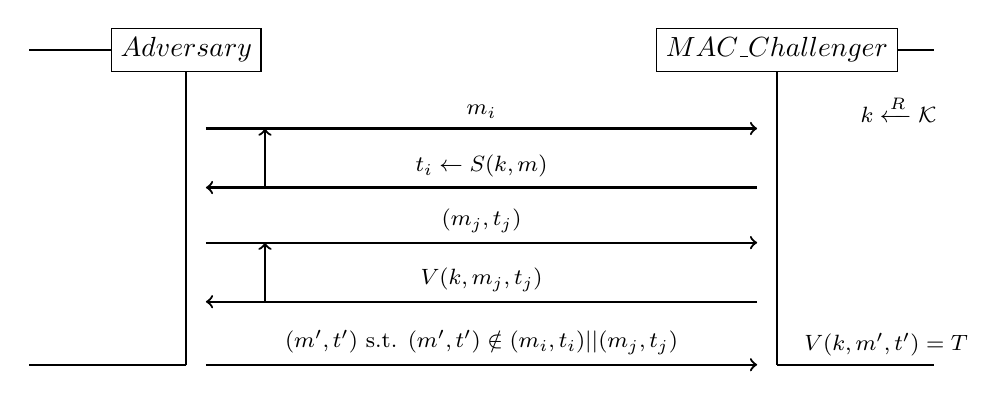
\begin{tikzpicture}
        \node[draw] (Adversary) at (-3, 2) {\(Adversary\)}; 
        \draw[thick] (Adversary) -- ++(0, -4); 
        \draw[thick] (Adversary) -- ++(-2, 0);
        \draw[thick] (-3, -2) -- ++(-2, 0);
        
        \pause

        \node[draw] (Challenger) at (4.5,2) {\(MAC\_Challenger\)}; 
        \draw[thick] (Challenger) -- ++(0, -4);
        \draw[thick] (Challenger) -- ++(2, 0);
        \draw[thick] (4.5, -2) -- ++(2, 0);

        \pause

        \node[draw=none,fill=none,anchor=east, font=\footnotesize] (choice0) at ($(Challenger) + (2.15,-.75)$) {\(k \xleftarrow{R} \mathcal{K}\)};

        \pause

        \draw[->,thick] ($(Adversary)+(0.25,-1)$) -- ($(Challenger)+(-0.25,-1)$) node [pos=0.5,above,font=\footnotesize] {\(m_i\)};

        \pause

        \draw[->,thick] ($(Challenger)+(-0.25,-1.75)$) -- ($(Adversary)+(0.25,-1.75)$) node [pos=0.5,above,font=\footnotesize] {\(t_i \leftarrow S(k, m)\)};

        \pause

        \draw[->,thick] ($(Adversary)+(1,-1.75)$) -- ($(Adversary)+(1,-1)$);

        \pause

        \draw[->,thick] ($(Adversary)+(0.25,-2.45)$) -- ($(Challenger)+(-0.25,-2.45)$) node [pos=0.5,above,font=\footnotesize] {\((m_j,t_j)\)};

        \pause

        \draw[->,thick] ($(Challenger)+(-0.25,-3.2)$) -- ($(Adversary)+(0.25,-3.2)$) node [pos=0.5,above,font=\footnotesize] {\(V(k, m_j, t_j)\)};

        \pause

        \draw[->,thick] ($(Adversary)+(1,-3.2)$) -- ($(Adversary)+(1,-2.45)$);

        \pause

        \draw[->,thick] ($(Adversary)+(0.25,-4)$) -- ($(Challenger)+(-0.25,-4)$) node [pos=0.5,above,font=\footnotesize] {\((m', t')\) s.t. \((m',t') \notin (m_i, t_i) || (m_j, t_j)\)};
        
        \pause

        \node[draw=none,fill=none,anchor=east, font=\footnotesize] (choice0) at ($(Challenger) + (2.55,-3.75)$) {\(V(k, m', t') = T\)};
      \end{tikzpicture} 
\end{frame}

\begin{frame}
  \frametitle{In Class Activity (20 minutes)}
  \text{Design a MAC based on a PRF}
\end{frame}

\end{document}
